% Chapter 1

\chapter{State of the art}

\label{State of the art}

%PAPER of ref: https://www.researchgate.net/publication/286649850\_A\_survey\_of\_botnet\_detection\_based\_on\_DNS 
\section{Botnets}
%[A survey of botnet detection based on DNS]Kamal Alieyan Ammar ALmomani Ahmad Manasrah Mohammed M. Kadhum
As stated in the introduction botnets are an important problem for anyone involved somehow with the internet. They can result in great economic damage.
%Authority of Information Security. The 2016 Vietnam Information Security Report; Authority of Information Security, MIC: New York, NY, USA, 2016.
Especially with their continuous improvement to become more resilient and powerful which makes them an even more important threat.\\\\
%http://dimva2014.isg.rhul.ac.uk/slides/phoenix-talk.pdf
Botnets can become very lucrative and can infect very large amounts of devices resulting in scary entities. Here are some of these enormous entities: \textbf{Flashback} with 600k compromised targets, \textbf{Grum} with 840k compromised devices and sending 40 Billion spam emails per month, \textbf{TDL-4} with 4.5 Million victims in first the 3 months and \textbf{Gameover ZeuS} with 1 Million infections, because of its resilience mechanisms this botnet was one of the hardest to take down.\\\\
%source 6 (A survey of botnet detection based on DNS) 
The reason botnets are still an ongoing research topic is that there isn't a complete solution for their detection and mitigation. Researchers and organisations have to keep working to keep updated with all the new flavors criminals bring to the market.
\subsection{Definition}
% WHAT IS A BOTNET?
%memoire1
%source Wielogorska, Monika and O'Brien, Darragh (2017) DNS Traffic analysis for botnet detection. In: 25th Irish Conference on Artificial Intelligence and Cognitive Science, 7-8 Dec 2017, Dublin, Ireland.
\paragraph{What is a botnet?} A botnet is a network of infected machines with programs called bots, these bots owned and controlled by a remote attacker called the botmaster. Users get infected via the same vector attacks used by malware, email attachment, malicious website, unaware download, etc. When bots usually infect these machines in stealthy manner, staying as unnoticeable as possible. The control of such bots is done through the Command and Control (CnC) server. The CnC server allows the master to issue commands to and receives responses from individual bots or aggregations of bots. These exchanges are done to update the software of the malware, execute attacks, exfiltrate data and more actions explained down below.
%https://arxiv.org/pdf/1702.01132.pdf

%WHAT IS A BOT?
%source http://www.honeynet.org/node/53
\paragraph{What is a bot?} Bots are small programs allowing to remotely control and perform commands on computers. They are the foundation of botnets. The paper presented by the SANS institute considers two types of bots. Bots used to perpetuate attacks, bots used for their content and both. % [Botnet Tracking Tools] SANS Institute 
%http://www.technicalinfo.net/papers/PDF/WP_Botnet_Communications_Primer_(2009-06-04).pdf
A clear distinction between a bot agent and a common piece of malware lies within a bot's ability to communicate with a Command-and-Control (CnC) infrastructure. CnC allows a bot agent to receive new instructions and malicious capabilities, as dictated by a remote criminal entity. This compromised host then can be used as an unwilling participant in Internet crime as soon as it is linked into a botnet via that same CnC.\\
These programs are embedded with port scanning, vulnerability scanning, exploitation kits and payloads that allow them to spread the botnet and infect their victims.\\
There are many different families of bots, some very modular such as the Agobot others less complete but easier to use such as the SDBot family. Bots families are also classified depending on the channel type and attack type, for example GT-Bots are a IRC bots but there are a lot of different protocols exploited as botnets channels. These 3 families are the most often found. Lesser usual ones have specific functions or plugins to fill in the gaps left by developers to customize the bots, a good examples would be the Dataspy Network X bots. There are very small bots such as the Q8 Bots and Perl-based bots that still allow for a large range of commands and attacks. Finally some bots are composed of a single file like Kaiten bot which makes it very easy to upload to compromised machines.

%WHY BOTS PROVIDE EVEN MORE POWERFULL ATTACKS
% S. S. Silva, R. M. Silva, R. C. Pinto, and R. M. Salles. Botnets: A survey. Eslervier, 57(2):378–403,2013
\paragraph{Why do botnets provide more powerful attacks?} Botnets give the control to the botmaster of two critical resources: CPU (processing power) and IP addresses (anonymity). Even if the use of CPU stays low on the infected machines, the aggregate of bots can provide power equivalent to supercomputers with the additional perk of executing traffic from different addresses instead of a single IP.

% PURPOSE + CURRENT DANGERS
\paragraph{What is the purpose of botnets?} All these resources make botnets very powerful to execute network attacks. 
%https://ccdcoe.org/cycon/2012/workshops/Intro_to_Botnets.pdf
Cybercriminals use botnets to execute a long list of malicious activities and structure related actions, we have listed some of these but any type of cyber attack can be uploaded to these bots and executed.
% + source http://www.honeynet.org/node/52

% ADVANCES IN BOTNETS
%source Emre Y (2011) A literature survey about recent botnet trends. http://geant3.archive.geant.net/Media_Centre/Media_Library/Media%20Library/botnet_trends_M2.pdf
\paragraph{What are the advances in botnets?} Another reason botnets are a big threat is that criminals have started to provide botnets as a Service (BaaS) which are considered a big part of the botnet economy. This popularized botnets are sold to anyone, this has made them an even bigger threat that they already were.
This BaaS is possible with decentralized architectures that can subdivided into smaller botnets to sold and then reintegrated to the parent botnet after use.
%source % [Botnet Tracking Tools] SANS Institute 

%memoire1
\paragraph{What types of actions are performed by botnets?} A victim host could be infected by targeting known vulnerability or by infected programs. When the victim is infected, the botnet will try to stay stealthy and with the exploit kit installed, it can do an extensive amount of damage. Here are some of the methods to control the infected hosts.\\
This first list presents general use of botnets:
\begin{itemize}[noitemsep]
\item \textbf{Distributed Denial-of-Service Attacks} These attacks provoke a loss of service or connectivity. Used by hacktivist, criminals and companies to disturb targets for recognition, financial gain or advantage over competition respectively. (The services could be email servers, production servers, web servers but also any device reachable) %source http://www.honeynet.org/node/52
\item \textbf{Spam email campaigns} Bots are set as proxy nodes and then used to send large amounts of spam and phishing emails.%source http://www.honeynet.org/node/52
\item \textbf{Sniffing Traffic} Bots can start watching packets going through the compromised machine and start retrieving all valuable data passed in clear-text. Botnets have been even found to analyze others bots data and take over them if they belong to another botnet.
\item \textbf{Spying through Keylogging and file monitoring} Sniffing packets effectiveness is reduced by encrypted traffic. The solution is then to log the key strokes made by the users and retrieve sensitive information. This is done with a keylogger and filtering mechanism that targets specific use-cases (logins, password, ...)%source http://www.honeynet.org/node/52
\item \textbf{Spreading new malware} Botnets growth depends on their ability to expand. Compromised targets have an important task to keep spreading the botnet. They can download malware or send viruses via email, there are various methods depending of the botnet type and environment they want to spread the malware.%source http://www.honeynet.org/node/52
\item \textbf{Installing Advertisement Addons, Browser Helper Objects (BHOs) and Google AdSense abuse} These techniques are used for financial gain instead of disruption. These are based on websites using clicking based ads. The criminals set fake sites using advertising programs and then automate the bots to click on them to create revenue. Since the bots have different IPs it is very hard to detect the fraud.
\item \textbf{Manipulating online polls and games} These are known to exist to influence decisions and are expected to be further used in the future. This is also very effective since each bot uses different IP addresses.
\item \textbf{Mass identity theft} Stealing personal data such as mail accounts, intellectual property, military secrets, embarrassing information or bank credential. This is a combination of all of the above that allow to create campaigns based on that data collected. These campaigns make this stolen data effective through fake websites and spear phishing email attacks. % [Botnet Tracking Tools] SANS Institute 
Regarding the personal information that can be found by bots on the home desktops, this paper explains that it must not be overlooked. The amount of data that can be contained in home applications can be very important(taxes, browsers, email contacts. They warn of the sensitive information that is often stored on home computers related to their company. This could expose intellectual property that can be then sold by the criminals.
\item \textbf{Host illegal sites} Child pornography and black market sites are some examples.
\item \textbf{Computation for cryptanalysis} This is a less expected use of botnets, but these distributed supercomputers can be used for cryptanalysis purposes. Computing rainbow tables, cracking passwords, bruteforcing keys or mining crypto currencies. With the success of cryptocurrencies in the last 2 years, this type of use for botnets has increased. The latest example is the Smominru Monero mining botnet, mining around 9000 moneros worth at the time 3 million\$.
%https://www.proofpoint.com/us/threat-insight/post/smominru-monero-mining-botnet-making-millions-operators+% [Botnet Tracking Tools] SANS Institute 
\end{itemize}
%A Survey on Botnet Architectures, Detection and Defences
This second list targets activities of bots on the compromised machines to take full control:
\begin{itemize}[noitemsep]
\item \textbf{Secure the system(close NetBIOS shares, RPCDCOM) to avoid infection by other criminals} This could also mean remove existing bots on the machine. Bots will make sure their host is properly hardened to avoid overtake.
\item \textbf{Redirect traffic for the botnet} Depending on the topology used, bots might be used as proxies to send commands, updates, data to the rest of the bots.
\item \textbf{Kill unwanted process running on the system} This joins the hardening objective. Bots want to take full control and make sure no process is limiting their actions (usually trying to stay stealthy while doing it).
\item \textbf{Test for virtual machines and/or debugger software} Part of the resilience of botnets resides in the obscurity of the mechanism they use. Honeypots will try to capture bots and do malware analysis to understand how they work. This tests will try to prevent this analysis to happen. (By deleting themselves or not executing in these environments)
\item \textbf{Add or delete auto-start applications} To stay resilient after reboot or even fresh installs, bots have mechanisms to stay persistent on the machine after those events.
\item \textbf{Run or terminate programs} This one is obvious but after exploiting the victim, their goal is to execute actions on the machine.
\item \textbf{Download and execute files} This allows them to update their software, download exploits and payloads. It can also be used to upload normal programs used for some of the tasks they want to execute.
\item \textbf{Perform address and port scan} Another important one to pivot inside networks and expand the botnet surface.
\item \textbf{Communicates with a handler or controller via public servers or other compromised systems} This is the  main channel communication with the botmaster.
\item \textbf{Data storage} One of the tactics used by botmasters to keep their anonymity is to use their botnet as a distributed database and saving the data obtained on the bots, this gives more distance with the stolen data.% [Botnet Tracking Tools] SANS Institute 
\end{itemize}

%\subsection{Structure}
%\subsubsection{Life cycle}
\subsection{Life cycle}
\paragraph{What are the steps that make up a botnet life cycle?} Life cycle execution might differ from one bot to another but they have generally a common structure. Here is te common structure presented in these studies: 
%A survey of botnet detection based on DNS
%[1] David Zhao, IssaTraore, BassamSayed, Wei Lu, SherifSaad, Ali Ghorbani and Dan Garant,”Botnet detection based on traffic behavior analysis and flow intervals,”Elsevier Computers & Security, vol. 39, pp. 2-16,November 2013.
%[2] Maryam Feily, AlirezaShahrestani and SureswaranRamadass,” A survey of botnet and botnet detection,” in2009Proc.IEEE third international conference on emerging security information, systemsand technologies, pp.268-273
%source Z. Zhu, G. Lu, Y. Chen, Z. J. Fu, P. Roberts, and K. Han, “Botnet research survey,” in 32nd Annual IEEE International Conference on Computer Software and Applications, pp. 967–972, Aug. 2008
\begin{enumerate}
\item \textbf{Exploitation} The first phase is the infection of the host. The bots gets access to the victim host through different possible vectors (email attachment, vulnerability scanning and exploit, obtained credentials, malicious site, ...). The next step of this phase consists on uploading to the host the binary of the bot. 
%25. Abu Rajab M, Zarfoss J, Monrose F, Terzis A (2006) A multifaceted approach to understanding the botnet phenomenon. In:Proceedings of the 6th ACM SIGCOMM conference on Internet measurement. ACM, pp 41–52
The bot connects to a server of the botmaster and downloads it. This step is very important for this thesis because it is the first DNS lookup the bot will perform and it has been noticed as the most consistent behavior of bots. This is where the bots are going to start to hide their DNS activity.
%26. Abdullah RS, Abdollah MF, Noh ZAM, Mas’ud MZ, Selamat SR, Yusof R, Melaka UTM (2013) Revealing the criterion on botnet detection technique. IJCSI Int J Comput Sci Issues 10(2):208–215
%16. Manasrah AM, Hasan A, Abouabdalla OA, Ramadass S (2009) Detecting botnet activities based on abnormal DNS traffic. arXiv preprint arXiv:09110487
%source P. Barford and V. Yegneswaran, “An inside look at botnets,” in Advances in Information Security, vol. 27, pp. 171–191, Springer, Mar. 2007
%source G. Gu, P. Porras, V. Yegneswaran, M. Fong, and W. Lee, “Bothunter: detecting malware infection through ids-driven dialog correlation,” in Proceedings of 16th USENIX Security Symposium on USENIX Security Symposium, pp. 1–16, Berkeley, CA, USA, 2007.
\item \textbf{Rallying} This is the phase where the bots will establish the link with the botmaster command and control servers (CnC), join the botnet and wait for instructions. When establishing the connection with the botmaster bots have to use stealth techniques to avoid getting discovered and more importantly revealing the CnC. These techniques will be discussed in the Misuses and abuses of DNS.
%18. Choi H, Lee H, Lee H, Kim H (2007) Botnet detection by monitoring group activities in DNS traffic. In: 7th IEEE international conference on computer and information technology, 2007 (CIT 2007). IEEE, pp 715–720
%27. Liu L, Chen S, Yan G, Zhang Z (2008) Bottracer: executionbased bot-like malware detection. In: Wu T-C, Lei C-L, Rijmen V, Lee D-T (eds) Information security. Springer, Berlin, Heidelberg, pp 97–113
\item \textbf{Attack/execution} From this point on the bot is ready to get the orders from the botmaster and start executing actions. This is where the different actions defined above are executed by the botnet.
%17. Rodrı´guez-Go´mez RA, Macia´-Ferna´ndez G, Garcı´a-Teodoro P(2013) Survey and taxonomy of botnet research through lifecycle.ACM Comput Surv (CSUR) 45(4):45
\item \textbf{Update and maintenance}
This phase allows the botmaster to update periodically the software of the bots, new exploits, new attacks, the same way administrators patch their software. This final phase is a loop that goes back to the second phase where the bot contacts the CnC server to proceed to this binary upload and commands fetching. This is the second phase where the DNS request will use evasion techniques to stay hidden.
% 6. Karim A, Salleh RB, Shiraz M, Shah SAA, Awan I, Anuar NB (2014) Botnet detection techniques: review, future trends, and issues. J Zhejiang Univ Sci C 15(11):943–983]
\end{enumerate}

\subsection{The Channel}
\paragraph{What does it mean to join the botnet?} The bots will rarely directly connect to the CnC servers, they will go through proxies or peers bots, (structural nodes of the botnet) to obtain commands and updates. The knowledge of these nodes and the techniques used to communicate with them are the channel of a botnet.
\paragraph{What are the channels used by botnets?} The channel's resilience of a botnet is critical to ensure good communication with the CnC server. It is also a critical component because its failure is usually the end of the botnet's life. There are multiple ways of securing and hiding their communication channel: tunneling through protocols, encryption, DNS evasion techniques.
%https://ccdcoe.org/cycon/2012/workshops/Intro_to_Botnets.pdf
The typical protocols that are used by bots to reach their CnC are these: IRC, HTTP, HTTPS, DNS, MAIL, SSH, etc. The use of different protocols implies there are a multiple botnet's communication topologies. The different topologies provide trade-offs in terms of bandwidth, rallying, stealth, ...

\paragraph{What are these different protocols ?}

\paragraph{What are the goals of these different channels?}
%http://www.technicalinfo.net/papers/PDF/WP_Botnet_Communications_Primer_(2009-06-04).pdf
The main goal of the botnet channel is to provide a vector for bots to reach their CnC servers and maintain a connection with it. This is the only way the botmaster is able to keep control his botnet. This is why the means of communication are built around these main needs. If bots aren't able to reach the botnet or their CnC, they won't be able to update their software and receive commands.\\ 
Reaching and locating the CnC servers is the first challenge the channel needs to handle. Failing to do so will leave the bot unusable for the botmaster or left in a sleeping mode. In this state, the bot keeps on with the harvesting of the victim host and retry the missed CnC regularly. \\
The second challenge being its ability to maintain the channel. This is where resilient techniques have evolved to achieve this goal. These technologies will be detailed in the abuses of DNS section. CnC servers and their channels are really what differentiates botnets from other malware. 
%ABOVE: J. Goebel and T. Holz, “Rishi: identify bot contaminated hosts by IRC nickname evaluation,” in Pro- ceedings of the first Conference on First Workshop on Hot Topics in Understanding Botnets, pp. 8, Berkeley, CA, USA, 2007. file:///D:/CyberSecurityMaster/Master%20Thesis/papers/Botnet_general/botnet_review.pdf
	
\paragraph{How do botnets achieve such channels?}
%BELOW: H. Choi, H. Lee, H. Lee, and H. Kim, “Botnet detection by monitoring group activities in dns traffic,” in The 7th IEEE International Conference on Computer and Information Technology, pp. 715–720, Oct. 2007.
%BELOW: “Taxonomy of botnet threats,” white paper, Trend Micro Incorporated, Nov. 2006. (http://www.cs.ucsb.edu/ kemm/courses/cs595G/TM06.pdf)
To stay invisible and persistent channels have gone through different methods, here are the main ones: 
\begin{itemize}[noitemsep]
\item \textbf{Hardcoded IP}: The bot software has the IP address of the CnC server hardcoded somewhere in its binary. The server can be found through reverse engineering and the botnet could be stopped or suspended for a certain period.
\item \textbf{Dynamic DNS}: This is a solution to the hardcoded IPs. In this case the botnet will have multiple CnC servers migrating frequently on its will. In addition to using a dynamic list of servers, it uses dynamic DNS in order to avoid detection or suspension and keep the botnet portable. This allows the queries to be redirected if they were to fail. This behavior is known as herding, it provides mobility and stealth.
\item \textbf{Distributed DNS}: To avoid law, botmaster locate their DNS servers outside of the law's jurisdiction. Bots have the addresses of the DNS servers and contact them to resolve the IP address of the CnC servers.
\end{itemize}

\subsection{Topology}
\paragraph{How are the channels used ?}
Now that we know the purpose of channels and what they provide to botnets we are going to explore the different topologies used by botmasters using different channels and architectures.

\paragraph{What are the different topologies used by botnets?}
%[A Survey on Botnet Architectures, Detection and Defences] Muhammad Mahmoud, Manjinder Paul Nir, International Journal of Network Security · January 2014 file:///D:/CyberSecurityMaster/Master%20Thesis/papers/Botnet_general/botnet_review.pdf
The differences between topologies are related to protocols of communication. Their structure will result as mentioned above in trade-offs for its different specifications.

%https://ccdcoe.org/cycon/2012/workshops/Intro_to_Botnets.pdf
As explained in this paper, there are two typical botnet topologies which all the other topologies are built on:
\begin{itemize}[noitemsep]
%http://www.technicalinfo.net/papers/PDF/WP\_Botnet\_Communications\_Primer\_(2009-06-04).pdf
\item \textbf{Centralized}: This is the simplest structure. The CnC is the center of the architecture, responsible directly of the data and command exchanges with the bots. This central unit operates the whole botnet. The main advantages is speed and simplicity, this makes it easier to plan attacks and arrange the botnet. The big problem is that the CnC is the single point of failure of the architecture. If it goes down, the whole botnet is rendered ineffective. The main protocols used are IRC(Internet Relay Chat) and HTTP(Hyper Text Transfer Protocol, the protocol used to communicate between browsers and web servers). IRC is a client-server application for text messaging. The reason it is used as CnC servers is because it can set communications anonymously, between one and multiple users and is very easy to setup. Using the HTTP started because IRC channels were becoming to popular and IRC detection systems were being put in place. But this isn't the only reason: HTTP allows to hide CnC servers behind normal web traffic. This is perfect to be invisible to firewalls and IDS(Intrusion Detection Systems). One of the differences between both lies in how the information is passed: with IRC CnCs bots receive flows of commands from their botmaster, HTTP CnC wait for bots action to send them the commands.
\item \textbf{Decentralized}: To avoid the single point of failure, botnet designers decided for a peer-to-peer (P2P) communication channel. This structure is much more resilient to detection and avoids the single point of failure. All bots are interconnected with each other and each one acts as client and server. New bots only need the addresses of some bots in the botnet to start communicating with the rest of the botnet. If parts of the botnet are suddenly offline or captured by authorities, the rest can still function normally and adapts rapidly to the situation.
\end{itemize}


%cf slide(11)(http://www.ijcttjournal.org/Volume4/issue-1/IJCTT-V4I1P104.pdf
\paragraph{What are the metrics used to assess these architectures?}
The important metrics for a botnet are a combination of the above sections:
\begin{itemize}[noitemsep]
\item Resiliency: The ability to resist different events such as the loss of nodes in the botnet, loss of a CnC, blacklisting of domain names, federal investigations, etc.
\item Latency: Reliability on the transmission of messages. The botnet provides the bots a protocol to ensure the transmission of messages without.
\item Enumeration: Accurately predict the botnet's size.
\item Defense: protection mechanisms against reverse engineering, static and dynamic analysis, virtual environment execution.
\item Financially: Its potential to be partitioned and sold into sub-botnets. 
\end{itemize}

Botnets have followed the evolution of the defenses they were up against, for this is reason botnet operators have now a large choice of architectures when it comes to create one. Botnets topologies have been optimized to sustain most defenses and allow for large remote oversee. The choice of topology will be largely influenced by the business model the botnet operator has in mind.

\paragraph{What are the different topologies?}
CnC topologies encountered in the wild typically match one of the following types:
\begin{itemize}[noitemsep]
\item Star
\item Multi-server
\item Hierarchical
\item Random
\end{itemize}
%source 
%Modeling Botnets architectures:
%diurnal propagation model %source D. Dagon, C. Zou, and W. Lee, “Modeling botnet propagation using time zones,” in Proceedings of the 13 th Network and Distributed System Security Symposium NDSS, 2006
%Super botnet model % source R. Vogt, J. Aycock, and M. J. Jacobson, “Army of botnets,” in Proceedings of Network and Distributed System Security Symposium (NDSS’07), pp. 111–123, Reston, VA, USA, Feb. 2007
%Stochastic P2P model %source E. Van Ruitenbeek and W. H. Sanders, “Modeling peer-to-peer botnets,” in Fifth International Confer- ence on Quantitative Evaluation of Systems, pp. 307–316, Sep. 2008 
%source “The möbius tool,” Apr. 2011. (https://www.mobius.illinois.edu/)
%advanced P2P hybrid model 
%source P.Wand, S. Sparks, and C. C. Zou, “An advanced hybrid peer-to-peer botnet,” in Proceedings of the first Conference on First Workshop on Hot Topics in Un- derstanding Botnets, pp. 2, Berkeley, CA, USA, 2007.

\paragraph{Star}
%http://www.technicalinfo.net/papers/PDF/WP\_Botnet\_Communications\_Primer\_(2009-06-04).pdf
The Star topology relies upon a single centralized CnC server to communicate with the rest of the botnet. Each bot agent is issued new instructions directly from the central CnC point. When a bot agent compromises a new victim, it is configured to reach its central CnC, where it will register itself as a botnet member and await for new instructions. The main problem with this topology is the single point of failure that constitutes the CnC server.

%https://ccdcoe.org/cycon/2012/workshops/Intro_to_Botnets.pdf

\paragraph{Multi-server}
Multi-server is the logical follow up of the star topology, it is the combination of star CnC botnets joined together with the CnC servers connected to eachother. This is close to what is done in cluster database management with multiple servers deployed for load balancing and data replication. This ensures that if a CnC server is removed from the botnet, the other CnC servers will take its load and manage the bots that were connected to it. This topology is more complicated to setup, botmasters can even add a geographical component by having these CnC servers in the countries with bots deployed to improve speed and improve resistance to legal shutdowns.

\paragraph{Hierarchical}
Hierarchical topology is a tree based structure where any part of the tree can be used as a botnet on its own. In this topology, bots can proxy the CnC commands and instructions to the rest of the tree. Another interesting aspect of this architecture is that bots do not know the location of the rest of the botnet. They are aware of parts of it. This allows makes it harder to take down the botnet and allows to segment it for selling or leasing. The downside of it is the latency of the botnet introduced by its branching rendering certain attacks difficult.

\paragraph{Random - P2P}
This structure is decentralized and is composed of dynamic master-slaves or P2P relationships. Any bot can be used as CnC by the botmaster and relay them to the rest of the bots. To be told apart from the other traffic going through the botnet, traffic with commands will have a specific identification as a signature. This topology is very hard to take down because any node can be used as CnC, it also hard to hijack because there isn't a central structure and communications between nodes don't always use the same paths. The weakness of this topology is that it can reveal a lot of information about the botnet by simply monitoring a infected node and its communications with external hosts.

TODO
\paragraph{Hybrid}
\paragraph{P2P}

\paragraph{What design to pick ?} Here is a summary of the features taken into account when creating a botnet.\\
\begin{tabular}{|p{7cm}|p{7cm}|}
\hline
Pros & Cons \\
\hline
\multicolumn{2}{|c|}{Star}\\
\hline
\textbf{Speed of Control} &\textbf{ Single point of failure}\\
The direct communication between the CnC and the bots allows data to be transferred rapidly & CnC blocked or otherwise disabled results in the botnet rendered ineffective.\\
\hline
\multicolumn{2}{|c|}{Multi-server}\\
\hline
\textbf{No single point of failure} & \textbf{Requires advance planning}\\
Load balancing and replication prevents it from happening and maintains control of the botnet. & To achieve an infrastructure that is resilient and balanced such as multi-servers demands further preparation.\\
\textbf{Geographical optimization} & \\
Geographical location of severs speeds up communications between bots where the CnC servers are situated and help with law take downs.&\\
\hline
\multicolumn{2}{|c|}{Hierarchical}\\
\hline
\textbf{Re-sale} & \textbf{Command latency}\\
The botnet's owner can segment the sections of their botnet for lease or resale to other criminals. & Because commands must traverse
multiple communication branches within the botnet, there can be a high degree of latency with updated instructions being received by bot agents. This delay makes some forms of botnet attack and malicious operation difficult.\\
\textbf{Hidden topology} &\\
Compromised bots don't know the structure of the botnet therefore they are unable to leak much information.& \\
\hline
\multicolumn{2}{|c|}{Random}\\
\hline
\textbf{Highly resilient} & \textbf{Command latency}\\
The decentralized infrastructure and the many-to-many communication links between bot agents make it very resilient to shutdown. & The random nature of communication links between bots adds unpredictability to the system which can result in high levels of latency for some clusters of bot agents.\\
& \textbf{Enumeration}\\
& The analysis of a bot and its exchanges reveals a lot about the botnet structure and components.\\
\hline
\end{tabular}

\newpage

%http://dimva2014.isg.rhul.ac.uk/slides/phoenix-talk.pdf
\section{Use and abuse of DNS protocol}
%source A survey of botnet detection based on DNS
The current trend of botnets is to hide their channel using the DNS services to hinder their identification and rallying process.\\

\subsection{DNS}
\paragraph{What is the DNS protocol ?}
The Domain Network System helps any device on the internet looking the location of a hostname (google.com) by providing its address (IP address).


Most of the time users send DNS requests with a particular question for the DNS server. The server will the reply a DNS responses, similar to the request with the "answer" field filled with the information requested. Here is the structure of the packets transmitted to help with the understanding of the sections used as features later on.
\subsubsection{The DNS protocol}
\paragraph{How does DNS work ?}
%https://ns1.com/resources/dns-protocol
When a client (user or device) tries to reach mail.google.com it sends a DNS request for that domain name from a \textbf{DNS client}.\\
The \textbf{DNS server} that receives the request will look in its records if he has it. If it does then it will send the address IP to the DNS client. Otherwise it will contact DNS name servers that could have the domain in their records following a specific logic in its search.\\
It will start by querying the \textbf{Root DNS servers} that will give it directions through the branches of the DNS tree hierarchy to the \textbf{Top Level Domains} DNS servers(TLD). It will first look for the TLDs resolving .com, then the name server that resolves google.com, down to the name server that will resolve mail.google.com to its IP address. The DNS server that received the first request will receive the response and send it to the client finally.\\
Finally, the client can now connect to the server using the resolved IP address.\\
\paragraph{Are there different methods to obtain the requested RR}
There are 2 methods of searching through the different DNS server from the \textbf{authoritative DNS} (DNS server assigned to or by the client DNS that will be queried first). It can be recursive or iterative. \textbf{Iterative mode} is an interaction between the authoritative DNS and all the other DNS servers where all request are initialized by it and all responses come back to it. \textbf{Recursive mode} is an interaction between DNS servers relaying the request and then coming back with the final answer. \\The Root DNS servers are always iterative, this has been set to avoid a DoS of those servers which could be caused if the were recursive. These servers are the backbone of the internet.\\
\\
\paragraph{What is the original purpose of DNS?}
The idea behind the protocol was to provide a human readable domain name to servers. That way humans could identify these domains and  associate them with something concrete. The protocol simply looks for the server with the lookup table transforming them into machine readable addresses.
TODO: show the Tree hierarchy of DNS
TODO: add a figure showing the protocol
(use %https://blog.superuser.com/2012/02/16/what-is-dns-and-which-server-do-i-choose/)
\paragraph{What are the most common use cases of the DNS?}
%http://www.iana.org/assignments/dns-parameters/dns-parameters.xhtml
The most know use case for DNS is the resolution of hostnames and domain names. DNS can ask a lot of different information related to a domain, this information is called Resource Record(RR).\\ Here is a list of the main RR and what they query.\\
\begin{itemize}[noitemsep]
\item \textbf{A}: translation of a hostname into an IP address.\\
\item \textbf{MX}: information regarding the mail servers of the domain queried (ex: DNS request for google.com with RR$=$MX could return mail.google.com) \\
\item \textbf{NS}: information about the DNS server used by that domain.\\
\item \textbf{TXT}: Text description of the domain queried.
\end{itemize}
\subsubsection{DNS message structure}
\paragraph{What is the format for the DNS messages exchanges between DNS clients and DNS servers ?}
\begin{verbatim}
    +---------------------+
    |        Header       |
    +---------------------+
    |       Question      | the question for the name server
    +---------------------+
    |        Answer       | RRs answering the question
    +---------------------+
    |      Authority      | RRs pointing toward an authority
    +---------------------+
    |      Additional     | RRs holding additional information
    +---------------------+

\end{verbatim}
The format of a DNS message is the same for a request or a response but parts of the message will be filled differently. In the request, the client will fill the \textbf{Question section} with the information that needs to be resolved:
\begin{verbatim}
                                    1  1  1  1  1  1
      0  1  2  3  4  5  6  7  8  9  0  1  2  3  4  5
    +--+--+--+--+--+--+--+--+--+--+--+--+--+--+--+--+
    |                                               |
    /                     QNAME                     /
    /                                               /
    +--+--+--+--+--+--+--+--+--+--+--+--+--+--+--+--+
    |                     QTYPE                     |
    +--+--+--+--+--+--+--+--+--+--+--+--+--+--+--+--+
    |                     QCLASS                    |
    +--+--+--+--+--+--+--+--+--+--+--+--+--+--+--+--+
\end{verbatim}
Here the client fills the values: \\

\begin{tabular}{c|l}
value & explanation\\
\hline
q\_name  & Domain name requested (domain to be asked) \\
\hline
q\_type  & Type of RR record requested (A,AAAA,CNAME,MX,NS,PTR,...) \\
\hline
q\_class & Class of the request (often IN for internet) \\
\hline
\end{tabular}

\paragraph{what is provided in the header section ?}
Here is a detailed description of the header of the DNS messages. 
\begin{verbatim}
	                               1  1  1  1  1  1
	 0  1  2  3  4  5  6  7  8  9  0  1  2  3  4  5
	+--+--+--+--+--+--+--+--+--+--+--+--+--+--+--+--+
	|                      ID                       |
	+--+--+--+--+--+--+--+--+--+--+--+--+--+--+--+--+
	|QR|   OpCode  |AA|TC|RD|RA| Z|AD|CD|   RCODE   |
	+--+--+--+--+--+--+--+--+--+--+--+--+--+--+--+--+
	|                QDCOUNT/ZOCOUNT                |
	+--+--+--+--+--+--+--+--+--+--+--+--+--+--+--+--+
	|                ANCOUNT/PRCOUNT                |
	+--+--+--+--+--+--+--+--+--+--+--+--+--+--+--+--+
	|                NSCOUNT/UPCOUNT                |
	+--+--+--+--+--+--+--+--+--+--+--+--+--+--+--+--+
	|                    ARCOUNT                    |
	+--+--+--+--+--+--+--+--+--+--+--+--+--+--+--+--+

\end{verbatim}
\begin{tabular}{l|p{10cm}}
value & explanation \\
\hline
identifier & id of request\\
\hline
opcode & Operation Type: 0 $\rightarrow$ query, 1 $\rightarrow$ Inverse query, 2 $\rightarrow$ DNS status\\
\hline
aa\_flag & Authoritative Answer: specifies if the responding server is an authoritative DNS server for the domain queried. \\
\hline
tc\_flag & Truncation: flag set on truncated messages due to length greater than that permitted.\\
\hline
rd\_flag & Recursion Desired: if set, asks the NS to pursue query recursively. This is opposed to the iterative method\\
\hline
ra\_flag & Recursion available: recursive query supported by NS\\
\hline
rcode  & Response Code: ignored in request, useful in answers to provide query information.(ex: type of errors)\\
\hline
questions\_count  & Number of entries in the Question section\\
\hline
answers\_count  & Number of RR in the Answer section\\
\hline
authority\_count  & Number of NameServer RR in the Authority section\\
\hline
additional\_count  & Number of RR in the additional section\\
\hline
\end{tabular}

\subsection{Botnets abusing DNS}
TODO: Present the different abuses of the DNS protocol to evade detection
(use previous descriptions but revisit writing and add more visualization and explanations on how exactly it works. (it is important for future arguments regarding the evasion methods. We need to inform our reader to be able to convince him later of our arguments)

\paragraph{why would botnets abuse the DNS protocol?}
Looking up the CnC servers of a botnet is an essential part in the lifecycle of a bot. To make this step more resilient, botmasters searched for multiple ways to lookup hostnames or play around them. This is where certain features of the DNS protocol became handy to fulfill that goal.
\paragraph{what features did they exploit ?}
Because of the growth of the internet, content providers have built complex infrastructures to sustain the load of the traffic and provide the best services. Some of the things implemented are load balancers, data replication, encryption, etc. To do so DNS has features that allow you to make the best of these types of architectures. These features have inspired the following misuses: fast-flux, domain flux and DNS tunnelling.

\subsubsection{Domain flux}
Domain-flux is a type of DNS feature where bots are equipped with a special Domain Generation Algorithm (DGA). This is then used to generate an ensemble of domains. The idea is to generate domains until one of them returns an IP address they can use to contact their CnC. The botmaster knows which domains are generated at a particular point in time since that is the seed of the algorithm and can register them before they are queried by the bots to be reached. This improves the resilience of botnets infrastructure a lot.

%http://www.technicalinfo.net/papers/PDF/WP_Botnet_Communications_Primer_(2009-06-04).pdf
\paragraph{There are the 2 techniques used to achieve domain fluxing}
TODO: rephrase this section
\begin{itemize}[noitemsep]
%https://kb.iu.edu/d/aiuv
\item \textbf{Domain Wildcarding} abuses the wilcarding capabilities of the DNS protocol. This can create rules that make all Fully Qualified Domain Names (FQDN) point to the same IP address. For a rule defined by *.example.com we would group all FQDN under that scope (mail.example.com, service.example.com, 123.example.com). DNS wildcarting is typical for phishing and spamming botnets, this allows to bypass some of the anti-spam defenses and even to use the wilcard argument as information to identify the new node (russia01.example.com, asdasdk.example.com).
\item \textbf{Domain Generation Algorithms(DGA)} is the latest technology used by botnets for domain flux. It consists of algorithms that generate domain names based on a seed (this is the changing factor in the algorithm, ex: current time) chosen by the botmaster. This creates a list of FQDN that changes constantly. Bots will try to reach all of the FQDN generated and when the botmaster wants to communicate with them, he will simply compute a couple of future FQDN and point them to his CnC servers to make them reachable by the bots and send the next instructions or updates. Since these domains only last a short amount of time, it becomes very complicated to block all of the possible generated domains.\\
% https://github.com/andrewaeva/DGA/tree/master/dga_algorithms
In this github repository, they have compiled some examples of DGA. As expected, the algorithms have 2 main functions, one that gets the seed (from input to the algorithm or using dynamic values such as date and time), the second is the domain generation, which will usually choose a TLD and then append the result obtained from the random function with the dynamic seed.
\end{itemize}

\subsubsection{IP flux}
%http://www.technicalinfo.net/papers/PDF/WP\_Botnet\_Communications\_Primer\_(2009-06-04).pdf
\paragraph{What is the concept of IP/Fast-flux networks?} A Fast-Flux Service Network (FFSN) allows to link a list IP addresses to 1 domain name. These addresses have a very short Time-To-Live(TTL) and are presented by packets in a Round-Robin fashion. The idea that DNS had behind this concept was to enable load balancing for Content Delivery Networks(CDN) to be able to point customers towards other nodes in the network to obtain the content sought. \\
    The network uses a combination of round-robin IP addresses and a very short  for any given particular DNS Resource Record (RR) to distribute a user’s request to a large number of compromised computers. The Fast-flux motherships are the controlling parts of the fast-flux service networks. It is very similar to the command and a control (CnC) system found in conventional botnets but provides more features. It is observed that these nodes are always hosting both DNS and HTTP services, for being able to manage the content availability for thousands of domains simultaneously on a single host. They collected information on the IP addresses assigned to the domain name and how those IP addresses (A and NS records) changed over time

%Survey on Botnets on DNS detection
\paragraph{why is IP flux so effective?} Unfortunately, botnets use the DNS traffic as any other legitimate host, which makes differentiating the legitimate DNS traffic from the illegitimate one a very challenging problem [16]. Moreover,botnet owners attempt to hide their communication with the bots to obstruct any deployed botnet detection processes [17]. The attackers or botmasters use the DNS services to hide their command and control (CnC) IP address ;to make the botnet reliable and easy to migrate from server to another without being noticed
%-----
Fast-Flux Service Network (FFSN) allows for one domain name to have an unlimited number of IP addresses, short TTLs(Time to live) values and the IPs rotating in a round robin fashion. IP addresses belonging to such a domain act as a proxy for any device attempting a connection with their respective
CnC server. This process helps botnet controllers avoid detection and blacklisting. But can be confused with real traffic. It has a different categories:
\begin{itemize}[noitemsep]
\item Single-flux: Multiple IP addresses are assigned to the same domain (either CNAME or A records). (low TTL, multiple autonomous system(AS) locations, proxies for master)
\item NS flux: Multiple NS records assigned to the same domain
\item Double-flux: Multiple name servers are assigned to the same domain and then use single-flux for the multiple IP addresses of the master. This provides a second layer of redundancy. This also means that the TTLs are short for the A records and the NS records too.
\end{itemize}

% file:///D:/CyberSecurityMaster/Master%20Thesis/papers/Botnet_general/botnet_review.pdf
Normal FF\\
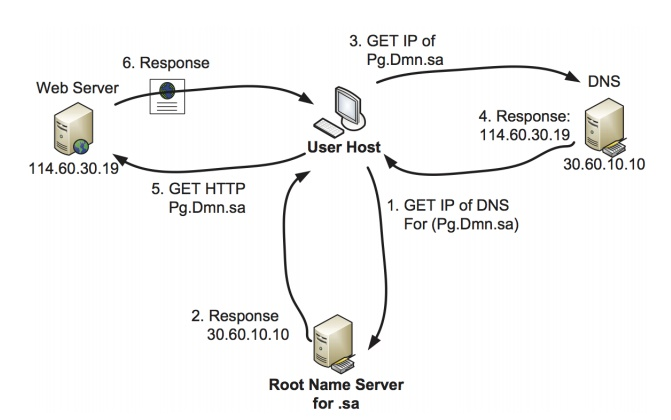
\includegraphics[scale=.7]{img/normal_FF.jpg}
single flux\\
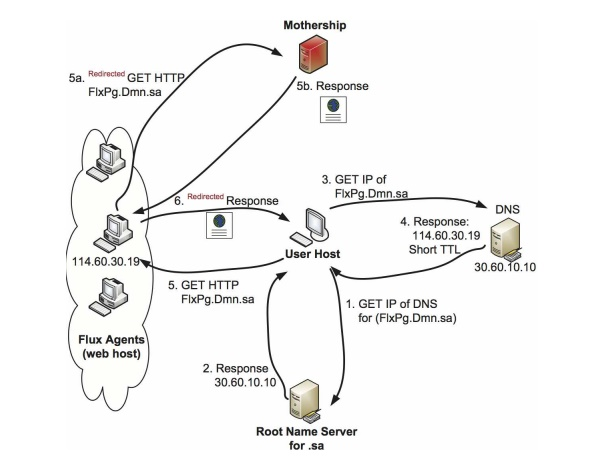
\includegraphics[scale=.7]{img/single_FF.jpg}
double flux\\
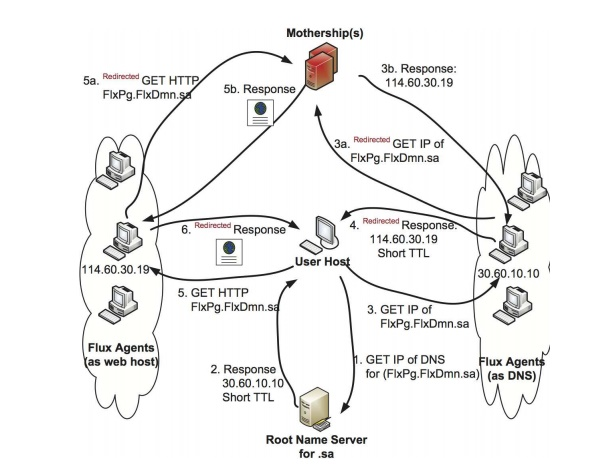
\includegraphics[scale=.7]{img/double_FF.jpg}

%source P. B¨acher, T. Holz, M. K¨otter, and G. Wicherski,“Know your Enemy: Tracking Botnets,” Oct. 2008. (http://www.honeynet.org/papers/bots)
This is done to allow the botnet’s domain name to have multiple IP addresses. In the meantime,
involved DNS records are constantly changing every few minutes using a combination of round robin
IP addresses and a very short TTL from any given particular DNS resource record.
In FFSN, the victim client first sends an address query to DNS. Then, the DNS returns the IPs of a
subset of active flux-agents. After that, the flux-agent relays the client’s request to the mothership3.
The key factor in FFSN is the combination of a very short TTL and the round-robin answer from a
large pool of active agents
%source P.Wand, S. Sparks, and C. C. Zou, “An advanced hybrid peer-to-peer botnet,” in
Proceedings of the first Conference on First Workshop on Hot Topics in Understanding Botnets, pp.
2, Berkeley, CA, USA, 2007.
Some features for FF detection: nb of A records returned: 1-3 normal, 5 or more ff nb of NS: normal
-> small, ff -> several NS + several A records for the NS AS: small nb of A from 1 AS -> normal,
located in different AS -> ff Hardware and IP: range of IP is diverged -> ff No physical agent -> ff no
guarantee uptime.
FIGURE NORMAL FF AND BAD FF (single and double)

DNS returns these A records in round-robin way.
CDN use a lower TTL to provide their content more efficiently
Fast-Flux Service Network (FFSN) is a distributed proxy network -built on compromised machines
(flux-agents)- that direct incoming DNS requests to the botnet’s desired address on the fly.
%source J. Nazario and T. Holz, “As the net churns: Fast-flux botnet observations,” in The 3rd International Con- ference on Malicious and Unwanted Software, pp. 24– 31, Oct. 2008.

\subsubsection{DNS tunnelling}
DNS tunnelling implies the act of tunnelling other protocols or data through DNS, for example using the TXT as q\_type and using the requests to actually send data. This has been done to avoid restrictions but is now also used to hide malicious traffic from botnets. They can also use DNS tunnelling to remain undetected while exfiltrating data. \cite{Botnet1}

\subsubsection{Maybe Domain shadowing (need more research)}
%[A Review Paper on Botnet and Botnet Detection Techniques in Cloud Computing] Shahid Anwar, Jasni Mohamad Zain, Mohamad Fadli Zolkipli, Zakira Inayat! Conference: ISCI 2014, September 2014
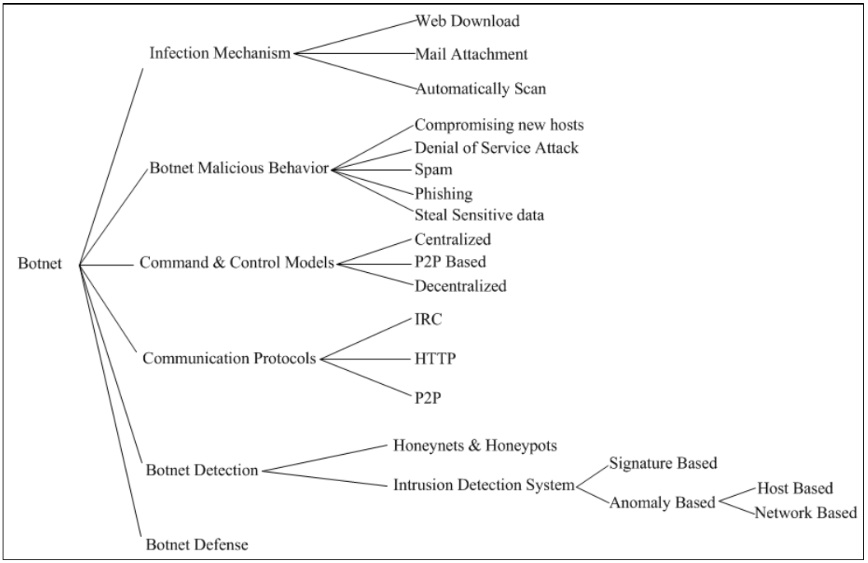
\includegraphics[scale=.8]{img/botnet_taxonomy.jpg}



TODO: Approches de base ML (classification, features selection,)
concepts généraux de machine learning qui vont être utilisés plus tard
afin d permettre le lecteur de comprendre. 

->elements de compréhension + preuve de la connaissance. 

% Botnet Detection Based On Machine Learning Techniques Using DNS Query Data, Xuan Dau Hoang and Quynh Chi Nguyen,  18 May 2018, MDPI, future internet
\section{Machine learning approach}
\paragraph{Machine learning} is a mathematical study of algorithms and statistics to improve the performance of specific tasks by building models of these problems. One of the tasks that machine learning algorithms excel at is the classification problem where the algorithms receive data as input and output to what group this data belongs to. Classification algorithms are very effective when it comes to detection problems, predictions, filtering.
\paragraph{why use machine learning for botnet detection?}
Because the botnet detection challenge presents itself as a great candidate for supervised and unsupervised classification algorithms. Supervised classification means that we have data that is labeled, in our case we have traffic that is know to be normal or malicious. On the other hand, for cases where the data isn't labeled we can group data that have common features(clustering) or detect anomalies in data that has features different from most of the group. 
\paragraph{How will ML be implemented for this Thesis}

\paragraph{What approach are we going to focus on and why}
\paragraph{What algorithms will be used }
\paragraph{what is the ML workflow}
%https://cdn-images-1.medium.com/max/2000/1*KzmIUYPmxgEHhXX7SlbP4w.jpeg

\section{Botnet detection related papers}
\subsection{classification of botnet research and detection}
In this section related to papers focused on Botnet detection, we are going to present the classifications of botnets and what part of the research we have decided to focus on.

%[Botnet Detection Based On Machine Learning Techniques Using DNS Query Data]
A number of botnet, detection measures, such as honeynet-based and Intrusion Detection System (IDS)-based, have been
proposed. However, IDS-based solutions that use signatures seem to be ineffective because recent
botnets are equipped with sophisticated code update and evasion techniques

Botnet detection and defense
Early bots detected through signature 
%source “SNORT,” Mar. 2006. (https://www.snort.org/)
-> vulnerable to any new botnet, but useful for old ones

%source D. Plohmann, E. Gerhards-Padilla, and F. Leder, “Botnets: measurement, detection, disinfection and defence,” in ENISA Workshop (Giles Hogben, ed.), Mar. 2011. botnet detection
classification: passive and active
%source “Taxonomy of botnet threats,” white paper, Trend Micro Incorporated, Nov. 2006. (http://www.cs.ucsb.edu/ kemm/courses/cs595G/TM06.pdf)
3 types of behavior: 
- network based behavior: observable network traffic between botmaster and bots, can be used to detect individual bots and their CnC server. 
- host based beavior: observable calls on the systems infected by botnets. 
- global correlated behavior: global behavior characteristics, structure will be similar to current structures; same for all mechanisms
%source H. Choi, H. Lee, H. Lee, and H. Kim, “Botnet detection by monitoring group activities in dns traffic,” in The 7th IEEE International Conference on Com- puter and Information Technology, pp. 715–720, Oct. 2007. 

"4.1.3 DNS Traffic Botmaster use DNS rallying to make their botnets invisible and portable. Choi et al. [20] proposed a botnet detection mechanism by monitoring their DNS traffic. Bots use DNS queries either to connect or to migrate to another CnC server. The DNS traffic has a unique feature that they define as group activity. Bots can be detected by using the group activity property of botnet DNS traffic while bots are connecting to their server or migrating to another server. There are three factors that help in distinguishing botnet DNS queries from legitimate DNS queries [20]; 
(1) queries to CnC servers come only from botnet members (fixed IP address space size), 
(2) botnet members migrate and act at the same time, which leads to temporary and synchronized DNS queries, 
(3) botnets usually use DynamicDNS (DDNS) for CnC servers. 
For a botmaster to keep its bots hidden and portable, he relies on DNS to rally infected hosts. In botnets, DNS queries can appear for many reasons. They appear during rallying process after infection, during malicious activities like spam or DoS attacks, during CnC server migration, during CnC server IP address change, or after CnC server or network link failure. Based on the aforementioned five situations of DNS query used in botnets, the authors have developed a Botnet DNS Q Detection algorithms, which distinguishes the botnet. This algorithm starts by building a database for DNS queries comprised of the source IP address, domain name and timestamp. Then, they group DNS query data using the domain name and timestamp field. After that, they remove redundant DNS queries. Finally, botnet
DNS queries are detected using a numerically computed some similarity factor [20] This algorithm cannot detect botnets migrating to another CnC server. Therefore, they developed a Migrating Botnet Detection algorithm by modifying the botnet DNS query detection algorithm. Similarly, this algorithm starts by building a database for DNS queries comprised of the source IP address, domain name and timestamp. Then, it groups DNS query data using the domain name and timestamp field.
After that, it removes redundant DNS queries. The next step will be to compare IP lists of different domain name with same size of IP list, because bots use two different domain names for the CnC server during migration [20]. These algorithms are protocol and structure independent and are capable of detecting unknown and encrypted botnets. However, these are not for real-time detections and have low accuracy for small networks. Furthermore, they are very sensitive to threshold values which need to be chosen very carefully to balance false positives and false negative rates.


% ========================================================================================

%source Botnet_Detection_Based_On_Machine_Learning_Techniques_Using_DNS_Query_Data
Honeynet: capture and analyze Pros: Easy to build, low ressources requirements Cons: Hard to
scale, limited interactions + can be reverted by hackers to learn new evasion techniques.
IDS: monitor and look for signs 2 types: signature or anomaly based through DNS analysis(most
promising) %source [ Botnet Detection Technology Based on DNS] Xingguo Li , JunfengWang ,and Xiaosong Zhang 
%source [A survey of botnet detection based on DNS] Kamal Alieyan • Ammar ALmomani • Ahmad Manasrah • Mohammed M. Kadhum
Anomaly detection approaches that work: 
- DNS Blacklist (for malware, botnets and spambots) 
%source [Revealing botnet membership using DNSBL counter-intelligence] Ramachandran, A.;Feamster, N.; Dagon, D.*
- detect botnets when they try to communicate with their CnC:
NXDomains 
%source: Villamari-Salomo, R.; Brustoloni, J.C. Identifying botnets using anomaly detection techniques applied to DNS traffic.
%source http://citeseerx.ist.psu.edu/viewdoc/download?doi=10.1.1.131.1318&rep=rep1&type=pdf
- recursive DNS queries detecting botnet related services %source: Perdisci, R.; Corona, I.; Dagon, D.; Lee, W. Detecting malicious flux service networks through passive analysis of recursive DNS traces
- DGA 
1) Main DGA %source: Yadav, S.; Reddy, A.K.K.; Reddy, A.; Ranjan, S. Detecting algorithmically generated malicious domain names. 
2) Decision tree + Bayes for DGA classification 
%source: Stalmans, E.; Irwin, B. A framework for DNS based detection and mitigation of malware infections on a network
- Kopis = high level DNS query analysis (upper hierarchy)
%source: Antonakakis, M.; Perdisci, R.; Lee, W.; Vasiloglou, N., II; Dagon, D. Detecting malware domains at the upper NS hierarchy
- Exposure 
%source Bilge, L.; Kirda, E.; Kruegel, C.; Balduzzi, M. Exposure: Finding Malicious Domains Using Passive DNS Analysis
graph analysis 
%source Jiang, N.; Cao, J.; Jin, Y.; Li, L.; Zhang, Z.L. Identifying suspicious activities through DNS failure graph analysis.
- reputation system 
% source Manos Antonakakis, Roberto Perdisci, David Dagon, Wenke Lee, and Nick Feamster. Building a Dynamic Reputation System for DNS

TODO: In the beginning we explain the detection classification proposed by the large survey. Then we explain what we have researched and how we'll use it in our work. Keep in mind that it isn't a list of papers, it is a list of information that will be used or not later in the paper, that has to cover that topics current research state and that we need to argue on reasons we want to keep articles or not and what information we'll use.
\\\\
After this presentation on the techniques used by Botmaster to set their botnets into certain topologies and evading the best they can current detection systems. We are now presenting the research papers that have tried to detect botnets using this different evasion techniques. Since the end goal is to find the best features for an all-in solution, we have structured the current state of research as follows: 
First we will present the current all-in solutions that exist, the features they extract and what model they have created. 
Secondly, to achieve our goal towards improving these solutions, the objective is to find better features and better models. We will present studies focused on single detection models that cover the field of detection through passive DNS analysis. For each study we will list the features proposed, understand their purpose and do a first selection if a thorough comparison has been made with the features presented. Otherwise they will saved for further analysis.
\\\\
In a recent survey of the state of the art regarding Botnet detection based on DNS traffic analysis\cite{survey}, they present a classification of botnet techniques (A survey of botnet detection based on DNS). They divide the classification into 2 categories, the honeynets and IDS(Snort). The later having evolved the most and where we want to focus. Most IDS were for a long time using signature-based techniques(check the IDS section for more details, p6). These are effective but only work with known botnets. Because they are signature-based there is a need to keep a blacklist updated very often, because a simple change creates a new signature and would be undetected if the database isn't updated with the latest signatures.\\
Newer techniques, described as "anomaly based" have emerged for 2 reasons: to detect unknown botnets and to respond to the new type of evasions that followed. Botnets have become a lot more resilient and stealthy. It has pushed the research to focus on features that would allow to distinguish between benign and malicious traffic.
These new researches capable of detecting new bots are divided into 2 sections: host-based and network-based. This means anomalies focusing on a single host or the traffic of a network. The host-based research focused on detecting bots in single hosts by monitoring local processes and kernel level routines.(BotSwat) The big problem of these propositions were the inability to scale them, we would need large monitoring system on each host with complex capabilities to communicate with each other and do correlation(EFFORT framework, the only one apparently. Do a bit more research on this framework and correct any mistakes in its previous description). This is what the second section aims to solve by monitoring networks. This activity can be done passively by simply collecting the traffic and analysing it (passive monitoring) or actively by injecting packets into the network forged to make the bots react, and then analyse the network response. 
Active monitoring: explain in more detail the rest of the approaches.
The part that our study focus on because "explain a valid reason for this part having more weight then the other ones, explain that our study could be a model combining different steps of the classification."
Finally explain the different passive approaches: 
\\
Explain that these passive detection can also be divided into specific counters for certain evasion systems such as DF, FF, tunnelling. Or be put together in an all-in solution to detect botnets independently of the evasion technique used.
\\
The first step in the research was to find the models that would be the current baseline for all-in solutions: Here we can start with 2 already gathered ones, and used the survey papers to find all-in solutions (if there are more than EXPOSURE), present them completely (features, dataset, model, purpose). 
IDEA: use the survey study chart to show strengths and weaknesses of papers.
\\
- Step needed before presentation of these papers:
classify them into the folders, 
create a summary for each one with the following information:
Model (data processing, dataset used, classification process, features)
finally for each relevant paper either do a summary with the 4 components or simple summary if redundant information.


After this part we are supposed to be done with the research, we have a last discussion of how the following step is planned and what information from this chapter will be translated into the rest of the thesis.



\subsection{All-in solutions}
\subsubsection{Exposure}

%[EXPOSURE: a Passive DNS Analysis Service to Detect and Report Malicious Domains] Leyla Bilge, Symantec Research, France Sevil Sen, Hacettepe University, Turkey Davide Balzarotti, Eurecom, France Engin Kirda, Northeastern University, USA Christopher Kruegel, University of California - Santa Barbara, USA.

\quote{EXPOSURE, a system that employs large-scale, passive DNS analysis techniques to detect domains that are involved in malicious activity. They use 15 features extracted from DNS traffic.}\\

\paragraph{Time-based}
When we analyse many requests to a particular domain over
time, patterns indicative of malicious behaviour may emerge.\\
These were supposed to be the features with the most weight, unfortunately due to lack of the same caliber of capture available to the authors of Exposure, we could not test out the 4 features related to time. Either because the datasets are compositions of smaller datasets, or because the timestamps are too short.
\paragraph{DNS answer based}
Here are some domain-flux features: A domain name can map to multiple IP addresses. In such cases,the DNS server cycles through the different IP addresses in a round robin fashion and returns a different IP mapping each time. \\
Malicious domains typically resolve to compromised computers that reside in different locations. The attackers typically use domains that map to multiple IP addresses, and IPs might be shared across different domains.
\begin{itemize}[noitemsep]
\item the number of different IP addresses that are resolved for a given domain during the experiment window
\item the number of different countries that these IP addresses are located in
\item the reverse DNS query results of the returned IP addresses
\item the number of distinct domains that share the IP addresses that resolve to the given domain (false positive can be reduced with google reverse DNS which will have hosting providers in top answers)
\end{itemize}
\paragraph{TTL value based}
Low TTL and Round-Robin DNS: \\
\begin{itemize}[noitemsep]
\item high availability (Content Delivery Networks (CDNs))
\item botnets using this, makes them resistant to DNS Blacklists(DNSBL) and take downs. Often using Fast-Flux Service Networks (FFSN).
\end{itemize}
Because FFSN are usually detectable because of low TTL and growing list of distinct IP addresses for a domain, it explains the purpose of the TTL features.
\paragraph{Domain name based}
Finally 2 simple features to expect detection of DGA: there is a big difference between legit domain names and domains generated by DGAs(Domain Generation Algorithms(DGAs).

This can be noticed with 2 simple features:\\
\begin{itemize}[noitemsep]
\item ratio numerical chars to length of domain name
\item length of the longest meaningful substring to length of domain name
\end{itemize}
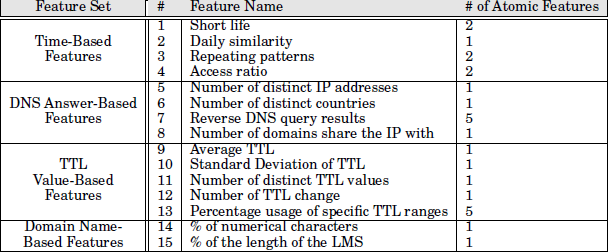
\includegraphics[scale=.3]{img/exposure_features.png}

\subsection{related papers}
\subsubsection{Domain-flux}
TODO: domain-flux can is mostly about analyzing domain names, here is a list of papers that attempt to do that with different metrics and features:  
%Detecting domain-flux botnet based on DNS traffic features in managed network Dinh-Tu Truong and Guang Cheng. https://de.wikipedia.org/wiki/Domain\_Flux, https://www.sciencedirect.com/science/article/pii/S1742287614001182, https://blog.malwarebytes.com/security-world/2016/12/explained-domain-generating-algorithm/\\
DGA specific\\
%Detecting Algorithmically Generated Malicious Domain Names, http://dimva2014.isg.rhul.ac.uk/slides/phoenix-talk.pdf

%
Domain flux is mainly used with DGAs and so here are some papers that have proposed an approach to detect it.

In \cite{dga}, they analyse the basic features that are common to most domain generated by DGA. The first is the length that can be an identifier because DGAs have long domain name. Recent DGAs have shown to have shorter lengths to blend with the other domains. They then propose 3 primitive features that capture linguistic and structural characteristics. They end with 2 more advanced features that cover the shortcomings of the primitive ones. They propose these features to detect DGAs:\\\\
\begin{tabular}{|l|}
\hline
length of the domain name excluding TLD (top level domain)\\
\hline
Number of vowels in the Second Level Domain (SLD)\\
\hline
Number of consonants in the SLD\\
\hline
Number of digits in the SLD\\
\hline
SLD trigram entropy\\
\hline
SLD trigram conditional probability\\
\hline
\end{tabular}
\\

These 6 features are very simple but have obtained really good results. The reason for the last 2 features is to improve the quality of the classification since some of the features could belong to botnets or legit domains. The definition of the features is explained in the section where this approach is analysed.

In this paper\cite{dga3}, they propose an unsupervised approach based on anomaly detection with a set of metrics analysing ngrams of the SLD. They use the Kullback-Liebler divergence measure with unigrams and bigrams, they also used the Jaccard index between bigrams and the last feature is the Edit distance. These 3 features are used widely in the DGA detection research because of their efficiency. \\

In this paper\cite{dga4}, they realize that during the generation algorithm, most of the domains will not be up, this will generate a lot of NXDomain responses. Furthermore, the caching of NXDomains is limited which means that they cannot hide this traffic. Their contribution consists of a clustering technique based on domain names and request patterns; and similarity metrics for malicious domains detection. What can be retrieved from this study is the feature related to NXDomains, and the clustering process for big datasets.

In \cite{phoenix}, they explain the shortcomes of some of the other approaches. The study works in 2 phases: DGA discovery and DGA detection. In the discovery phase they apply the following filters that focus on linguistics: percentage of meaningful word in the domain name; popularity of the ngrams of the domain. They construct a base generated with the top 100.000 domains from Alexa. Then they define a distance (Mahalanobis distance) and thresholds(loose and stric ones) to determine when domains can be considered DGAs. They use known malicious domains to determine their thresholds. Afterwards they propose a sytem to cluster DGAs. They create a graph where each node is a domain and edges are created if both nodes resolve to similar IPs, the weight is proportional to the number of common resolved IPs. From all the "communities" discovered, they extract different common features to be reintroduced in the detection phase for each family of DGAs.
%%%%%%%%%%%%%%%%%%%%%%%%%%%%%%%%%%%%%%%%%%%
\subsubsection{Fast-flux}
%memoire
%%%%%%%%%%%%%%%%%%%%%%%%%%%%%%%%%%%%%%%%%%
For IP flux, most papers have similar features they propose to detect fast-flux. The big challenge is to find the small differences and detect malicious fast-flux networks(FFSN) from content delivery networks(CDNs). Both use fast-flux for different reasons such as load balancing, high availability and evasion.\\
The features most papers \cite{honeynet}\cite{ff2}\cite{ff3}bring forward are shown on the figures below\cite{ff_botconf}, and listed here:\\\\
\begin{tabular}{|l|}
\hline
Numerous unique A records for a domain\\
\hline
Numerous unique NS records for a  domain\\
\hline
Different Autonomous Systems (ASN) for the IPs of linked to the same domain\\
\hline
Different countries for the IPs of linked to the same domain\\
\hline
Short Time-To-Live (TTL)\\
\hline
\end{tabular}
\\\\\\
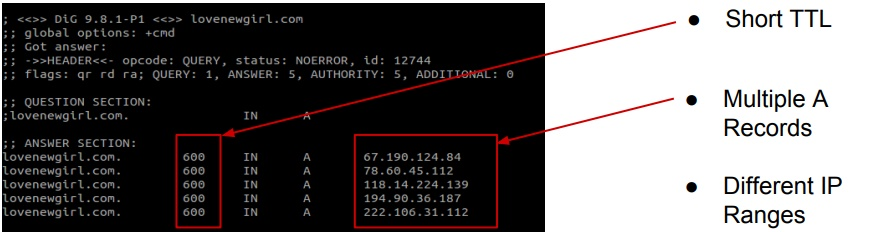
\includegraphics[scale=.7]{img/ff_features.jpg}\\
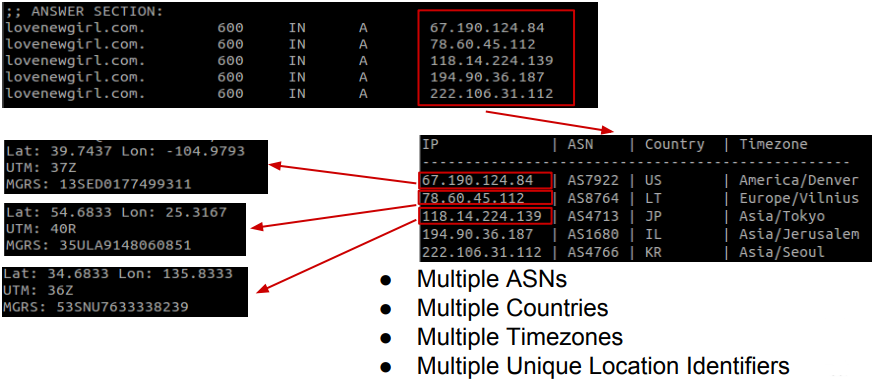
\includegraphics[scale=.6]{img/ff_features_2.png}
\\We present now the different features and approaches proposed to distinguish the CDNs from FFSN.\\

Before the approach taken by \cite{ff2}, most of the detection was based on DNS Blacklisting (DNSBL), their new approach was a passive analysis of recursive DNS traffic. Recursive DNS  when your query is send to your DNS server, it starts by checking its cache and then will recursively ask other DNS servers until finding the address. Their purpose was to allow direct analysis of DNS requests and detect malicious ones. They want to improve the HoneyNet\cite{honeynet} features(short time-to-live (TTL), set of resolved IPs returned at each query changes rapidly, usually after every TTL, the overall set of resolved IPs obtained by querying the same domain name over time is often very large, the resolved IPs are scattered across many different networks)\\
They start by applying filters to cluster the different networks of FF using the list above. On these clusters they then applied statistical supervised algorithms to do the classification. They used a base of features provided by \cite{fluXOR} and added their own. \\It starts with the passive features: \\\\
\begin{tabular}{|l|}
\hline
Number of resolved IPs\\
\hline
Number of domains (in a cluster = domains with similar IPs)\\
\hline
Avg. TTL per domain in a cluster\\
\hline
Network prefix diversity = ratio between the number of distinct\\ /16 network prefixes and the total \\
\hline
number of IPs (measures the scattering)\\
\hline
Number of distinct domain names that resolved to at least one of \\the IP addresses in the considered cluster\\
\hline
IP Growth Ratio. This represents the average number
of new IP\\ addresses discovered per each DNS response related to any domain\\
\hline
\end{tabular}
\\\\
Then the active ones:\\\\
\begin{tabular}{|l|}
\hline
Autonomous System (AS) diversity (ratio between the number of distinct\\ ASs where the IPs of a cluster reside and the total number of resolved IPs. \\Same for the following diversities)\\
\hline
BGP prefix diversity\\
\hline
Organization diversity\\
\hline
Country Code diversity\\
\hline
Dynamic IP ratio (ratio of dynamic vs total IPs using keywords in reverse\\ DNS lookups)\\
\hline
Average Uptime Index (average uptime for the IPs in a cluster,\\ Uptime tested through probing)\\
\hline
\end{tabular}
\\\\
They use these features on a Decision Tree classifier (efficient, easy to interpret and auto pruning of useless features) to classify malicious and legit FF networks.\\

In the following paper\cite{ff3}, they propose some novel features compared to the other papers. To avoid redundancy, only the features not explored in previous papers will be detailed. In the paper they present the restrictions FFSNs face compared to CDNs: FFSN cannot choose the location which makes the IP address very scattered and no Uptime garantee. Possible distinctions: the lack of control results in number of unique A records returned different and the number of NS records in a single lookup (because the NS can be hosted inside the FFSN and return many NS records whereas legitimate CDNs return a very small set of NS records). The IP diversity restriction brings another feature which is the number of unique ASNs. Legitimate CDNs tend to return a single ASN for all their A records where FFSN are dispersed.\\
They decide not to include TTLs as a feature because both CDNs and FFSN have low TTLs. Finally,  they introduce functions of the different features above to classify FFSN and CDNs.\\
\textbf{Fluxiness} is the total of unique A records for a domain divided by the number of A records returned for each lookup. This measures consistency in the unique A records returned. \\
\textbf{Flux-score} an hyperplane that separates benign from malicious fast flux where $ x = (n_A,n_{ASN},n_{NS})$ (unique A records, ASN and SN records) and the plane is defined as follows\\
%\begin{equation}
%F(x) = 
%\begin{cases}
%	w^Tx-b > 0  & \text{x is a FFSN}\\
%	w^Tx-b \leq 0 & \text{x is CDN}\\
%\end{cases}
%\end{equation}
From $F(x)$ they induce a metric $f(x) = w^Tx$ with w the weight of the vector and b a bias. $f(x) > b$ would mean x is a FFSN. By empirically testing this on a labelled dataset they determined the value of w and b. $w = (1.32,18.54,0)$ and $b =142.38$. We can notice that $n_{NS}$ does not have any impact. It could be argued that FFSN will try to mimic CDNs to have the same metrics, but as argued earlier, the metrics used take into account the restrictions FFSN have. The rest of the study approaches the detection of FFSN using the HTML content returned by the spam websites.\\

%Detection of Fast-flux Networks using Various DNS Feature Sets
This paper\cite{ff5} regroups the large majority of features encountered in the other papers accompanied with to some novel additions resulting a long list of 16 features: \\\\
\begin{tabular}{c|l}
Type & Features\\
\hline
 & Number of unique A records\\
DNS Answer-based &  Number of NS records\\
 & DNS packet size\\
 & TC (Tnmcated) Flag is set\\
\hline
 & Edit Distance\\
Domain name-based & KL (Kullback-Leibler) Divergence (unigrams and bigrams)\\
 & Jaccard Index (unigrams and bigrams)\\
\hline
 & Time Zone Entropy of A records\\
Spatial-based & Time Zone Entropy of NS records\\
 & Minimal service distances (mean and standard deviation)\\
\hline
 & Number of distinct autonomous systems\\
Network-based & Number of distinct networks\\
 \hline
 & Round Trip Time of DNS request\\
Timing-based & Network delay (mean and standard deviation)\\
& Processing delay (mean and standard deviation)\\
& Document fetch delay (mean and standard deviation)\\
\end{tabular}
\\

%%%%%%%%%%%%%%%%%%%%%%%%%%%%%%%%%%%%%%%%%%%%%

\subsubsection{DNS tunnelling}
%memoire
%%%%%%%%%%%%%%%%%%%%%%%%%%%%%%%%%%%%%%%%%%%%%%%
In \cite{tunn1}, use of TXT RR with segmented and encrypted data.
Rdata features: we look for the Shannon entropy of the strings. Measures the randomness of the string. Since encrypted data as a high level of entropy this is one of the things we'll be looking for. We are looking for "high byte entropy".Because of inherent reasons this entropy for a small string can't reach the max, we are looking at the "statistical byte entropy" instead.

The complete list of features for the Rdata:
\begin{itemize}[noitemsep]
\item number of distinct byte values in m
\item minimum byte value in m
\item maximum byte value in m
\item number of ASCII capital letters (byte values 65-90) in m
\item number of ASCII digits (byte values 48-57) in m
\item length of m in bytes
\item absolute difference of the statistical byte entropy at given length of m and the entropy of m
\item size of all Rdata messages
\end{itemize}
They expect these behavioural communication features to be effective enough in order to extend a classifier based on the rdata features.
\\\\
In this paper\cite{tunn}, they propose a visual approach to detecting DNS tunnelling, by plotting the following features, you can detect by "visual anomaly detection" the presence of DNS tunnelling. The features are:
\begin{itemize}[noitemsep]
\item x-axis: destination IP
\item y-axis: character count
\item radius: hostname length
\item colour: request type
\end{itemize}


%(cf Detecting DNS tunnelling)
%DNS has been used as a communication method by malware. Known malware
%using DNS include: Feederbot (Dietrich, 2011) and Moto (Mullaney, 2011). Both of
%these malware examples use DNS TXT records for command and control.
%%%%%%%%%%%%%%%%%%%%%%%%%%%%%%%%%%

\subsubsection{Behavioral}




